\section{Robot 1}

	\begin{figure}[h]
	\centering
	\subfloat[Figura de Matlab Robot 5.]{%
		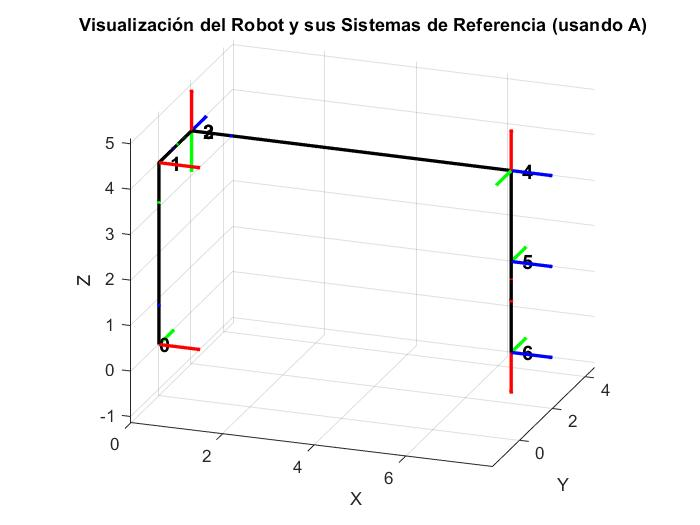
\includegraphics[width=0.45\textwidth]{ROBOT5MATLAB.jpg}%
		\label{fig:Interruptores de Limite}
	}
	\hspace{0.5cm} % Espacio entre imágenes (ajusta el valor si es necesario)
	\subfloat[Diagrama de lineas Robot 5.]{%
		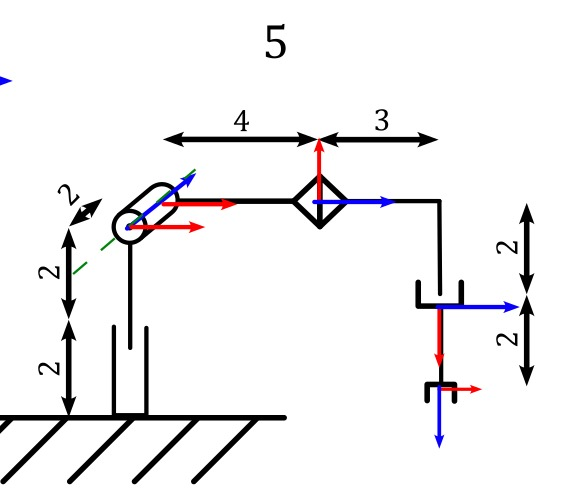
\includegraphics[width=0.45\textwidth]{DIAGRAMAROBOT5.jpeg}%
		\label{fig:FuncionamientoPiezoeléctrico}
	}
	\caption{Ejercicio 5 de Denavit Hartenberg.}
	\label{fig:PiezoeléctricoGeneral}
\end{figure}